\chapter{Data and Methods}

\section{Overview}

The purpose of this study is to develop a set of tools to allow the classification of agricultural crops using a time series of imagery and known crop reference signatures and test the portability of the reference signatures. The data used for this study consists of the following:

\begin{Spacing}{1.5}
\begin{itemize}
  \item 250-meter MODIS 16-day Composite Vegetation Index images
  \item 30-meter 2012 USDA Cropland Data Layer (CDL): agricultural land cover raster dataset
  \item 30-meter Landsat 8 Operational Land Imager satellite imagery
  \item Shapefile of the administrative boundary of the Department of Pellegrini \todo[inline]{CITE DATA SOURCE}
  \item 2014 Land cover vector dataset with crop identifications for Pellegrini
\end{itemize}
\end{Spacing}

The first two datasets are publicly available from US agencies. The land cover dataset for Pellegrini was digitized from Landsat 8 images, and the crop identifications were collected in the field.

An outline of the processing workflow is below:

\begin{Spacing}{1.5}
\begin{enumerate}
  \item Reproject the MODIS composite imagery
  \item Assemble individual composite images into single time series images, one for Kansas and one for Argentina
  \item Create a mask of all pure pixels (e.g. non-mixel) in the time series images
  \item Use the CDL to isolate the pure corn, soy, and sorghum pixels in the Kansas time series image.
  \item Identify the unique groups in each set of isolated pixels using k-means clustering
  \item Extract the pixel values for each cluster from the time series image and find the mean value for each date to find the unique signatures for each crop
  \item Validate the signatures by fitting the signatures to the time series image, then classifying the fit rasters to check the accuracy
  \item Fit the signatures to the Argentina time series image
  \item Classify the Argentina fit rasters and assess the accuracy
\end{enumerate}
\end{Spacing}

This chapter is a look at the theory and concepts behind this classification approach, the methods used to create the validation land cover dataset of Pellegrini, and the data processing steps used to generate the study results. Details about the specific tools in the classification toolset and the development process can be found in Appendix \ref{appendix:tools}. For a detailed explanation of all the testing proceeding this study, please see Appendix \ref{appendix:testing}. A thorough recounting of my field experience can be found in Appendix \ref{appendix:fieldwork}.

\section{Composite Vegetation Indices and Time-Series Images}

The differentiation of crop types in remotely-sensed imagery is not a straightforward process. The use of a vegetation index (VI), such as the normalized difference vegetation index (NDVI) or the enhanced vegetation index (EVI), can help identify crops by their specific VI values in an image.

NDVI is a normalized ratio of the red and near-infrared bands, and can be expressed mathematically as:
\begin{equation}
  NDVI = \frac{\rho~_{NIR} - \rho~_{red}}{\rho~_{NIR} + \rho~_{red}}
\end{equation}
where $\rho~_{NIR}$ and $\rho~_{red}$ are the measured surface reflectance in their respective bands. As a ratio, the index minimizes multiplicative noise, but has issues with non-linearity and additive noise \autocite{huete2002overview}.

With advances in calibration, atmospheric correction, and other noise removal techniques, which are integrated into the MODIS data processing workflow, a ratioing index is less necessary. The EVI was specifically developed for the MODIS platform to help correct some of the deficiencies of the NDVI. It has better sensitivity to high biomass, canopy structure, and leaf area, and less susceptibility to atmospheric degradation. EVI is calculated as:
\begin{equation}
  EVI = G\frac{\rho~_{NIR} - \rho~_{red}}{\rho~_{NIR} +  C_1\times\rho~_{red} - C_2 \times \rho~_{blue} + L}
\end{equation}
Again, each $\rho$ is the measured surface reflectance in the respective band, after complete or partial atmospheric correction. The blue band is used to ``subtract'' aerosol effects from the red band. Additionally, four coefficients are introduced: $G$ is the gain factor, $C_1$ and $C_2$ are used in the aerosol calculation, while $L$ ``is the canopy background adjustment that addresses nonlinear, differential NIR and red radiant transfer through a canopy'' \citereset\autocite[196]{huete2002overview}. The values of these coefficients as used in the MODIS EVI calculation are 2.5, 6.0, 7.5, and 1.0, respectively.

Some crops, such as soy and sugarcane, have very different spectral reflectance throughout their development and maturation, however others, such as soy and corn, can have very similar reflective curves, leading to overlapping VI ranges \autocite{price1994how-unique}. Such overlap can make it impossible to determine a crop type with specificity using traditional approaches; even using hyperspectral data, few differentiating characteristics between crops can hinder classification. To combat this ambiguity, a time series of images can be used to find VI values throughout a year, allowing the development of a classifier based on annual phenology rather than a single-date image \autocites{gu2010phenological}{wardlow2002discriminating}{wardlow2005state-level}{wardlow2007analysis}{wardlow2008large-area}{zhang2003monitoring}.
	
MODIS 16-day VI composite imagery from both the Terra and Aqua Earth Observing System (EOS) satellites is available from the Land Processes Distributed Active Archive Center (LPDAAC).\footnote{For those interested in working with MODIS data, the web address of LPDAAC is https://lpdaac.usgs.gov/, though data is not directly available from their servers without an exact link. I found the best tool for searching the available data was NASA’s Reverb|Echo web tool, at https://reverb.echo.nasa.gov/. Using this tool, one can get a list of links in a text file, and can use wget or curl to bulk download the files in the list.} Each MODIS satellite images the entire Earth daily: the Terra satellite makes its passes in the morning, while Aqua follows in the afternoon. This temporal resolution is the greatest advantage of the MODIS platform, as the likelihood of getting enough cloud-free data to develop a phenologic model is significantly increased over other common platforms like Landsat Thematic Mapper (TM) and Landsat Operational Land Imager (OLI), which only have repeat coverage every sixteen days. MODIS data, however, comes at the price of a reduced spatial resolution of 231 meters\footnote{Though the literature typically denotes MODIS data as 250-meter, the composite vegetation indices are actually 231-meter. However, to stay consistent with conventions, I will refer to the data as 250-meter.} compared to Landsat’s 30-meter pixels. At this resolution, crop mapping is restricted to medium farms and larger---those with fields of at least 250 meters square, though often a field must be up to two times larger in one dimension to ensure a pure pixel can be isolated. For the purposes of this investigation, however, this limitation is inconsequential, as small farms have a relatively minor impact on deforestation due to their size. Moreover, the crop of interest, GM soy, is only profitably grown using highly mechanized, input-intensive agricultural practices at very large scales. Small fields do not have high enough yields to overcome the significant capital investment required. [TODO: NEED A SOURCE FOR THIS---TALK TO POLO].

LPDAAC creates the VI composites using the maximum VI value over the proceeding 16-day time period. The images are numbered by the day of the year (DOY) of the last date in the image, so an image from DOY 17 is the composite of the images from January 2 through January 17.\footnote{Following this pattern exactly will make the first image from the following year be from January 4, but the MODIS composite numbering ``resets'' at the end of each year. Thus the image interval at the end of the year is shortened, allowing the next image to be produced January 1, though it still covers the proceeding 16 days.} Both NDVI and EVI are included in the MODIS VI products, and require no preprocessing for immediate use (unless cloud cover is pervasive in the area).

For this study, I chose to classify the 2012 Kansas summer growing season and the 2014 Argentina summer growing season. I assembled the MODIS 16-day composite VI images into multi-date time-series images (TSI) covering the growth cycle of the summer crops, where each band in a TSI is a 16-day composite VI, and the bands are ordered consecutively (see Appendix \ref{appendix:tools:build} for the description of the Build Multidate Image Tools) \todo[inline]{SHOW AN EARLY SEASON AND LATE SEASON VI SIDE-BY-SIDE TO ILLUSTRATE HOW VI VALUES DIFFER THROUGHOUT THE YEAR}. The Kansas summer TSI covered the date range DOY 97 through DOY 273, and was made with data from the Terra satellite. Prior to creating the TSIs, each of the 16-day composites was reprojected from the native MODIS sinusodial reference system using LPDAAC's MODIS Reprojection Tool \todo[inline]{CITE THIS TOOL}. I reprojected the Kansas data into the Albers Equal Area Conic projection for the contiguous USA using the 1983 North American Datum (WKID: 5070) to match the reference system of the USDA CDL.

In Argentina, as it is in the Southern Hemisphere and the seasons are inverted to those of the Northern hemisphere, the growing season shifts, as must the date range for the VI time-series. The TSI for Pellegrini must begin at the end of the proceeding year to adequately capture the entirety of the summer phenologies. To accomplish this, the time-series image for summer 2014 began with the 16-day composite image from DOY 345 of 2013 (or DOY −20 with reference to 2014) and ended with the image from DOY 105 of 2014. This specific date range was chosen based on information provided by local farmers to ensure coverage of the earliest planting and latest harvesting dates, as well as manual inspection of pixel signatures throughout the study area. Data through DOY 129 would have been preferred, but persistent clouds prevented using that late-date composite and necessitated the switch to the Aqua satellite's imagery. The Argentina composite images were reprojected with the UTM Zone 20S reference system (WKID: 32720).

\section{Crop Phenologies and Phenological Classification}
\label{chapter:methods:phenology-fitting}

\citeauthor{gu2010phenological} outlined that phenological statistics regarding vegetation development can be derived from a MODIS VI time-series, including “start-of-season time (SOST), start-of-season NDVI (SOSN), end-of-season time (EOST), end-of-season NDVI (EOSN), maximum NDVI (MAXN), maximum NDVI time (MAXT), duration of season (DUR), amplitude of NDVI (AMP), and seasonal time integrated NDVI (TIN)” \mkbibparens{\citeyear[529]{gu2010phenological}}. A principal component analysis (PCA) can then be used to extract the meaningful variation in the data. Similarly, Wardlow, Egbert, et al. \autocites{wardlow2002discriminating}{wardlow2005state-level}{wardlow2007analysis}{wardlow2008large-area} showed that a decision tree classifier can be used to classify vegetation time-series data into increasingly refined categories until specific crop types are isolated and classified. By beginning with a basic land cover classification (e.g. forest, urban, agriculture), crops in the agriculture class can be broken down into winter and summer varieties using peaks in the vegetation index (winter wheat will peak earlier in the year than summer crops like corn and soy). Then, using training sites of known crop types defined by ground truth data, a final crop classification can be assigned by finding pixel values for key dates where like crops can be differentiated. That is, using the growing season in the Northern Hemisphere as an example, if from the training sites we know crop A has VI values between 0.7 and 0.8 on June 26 and between 0.5 and 0.6 on August 29, while crop B is between 0.55 and 0.65 and 0.75 and 0.85 on the same dates, pixels in the summer crop class can be assigned one of these types by testing their pixel values on these dates. While the authors found this method to have about an 85 percent overall accuracy \autocite{wardlow2005state-level}, the downside of this method is that it requires training sites with previously-determined crop types to produce a classification, which can be time consuming and expensive to acquire.

\textcite{masialeti2010a-comparative} found that VI values from one year have a significant correlation with values from other years. Comparing the phenological curves of crops formed by the NDVI values from 2001 MODIS data \autocite[from][]{wardlow2005state-level} with those from 2005 MODIS data, the authors found the overall shape of each crop's curve is maintained year-to-year, with a subtle shift in the beginning of the curve (earlier or later planting), a scaling of the maximum of the curve, and and scaling of the spread of the curve (a longer or shorter growing season), depending on weather and other external variables (Fig. \ref{fig:transformations}). They surmised, with a means to account for the shift and scaling of the curve, one could use VI values from one year to classify those from another.

\begin{figure}
  \centering
  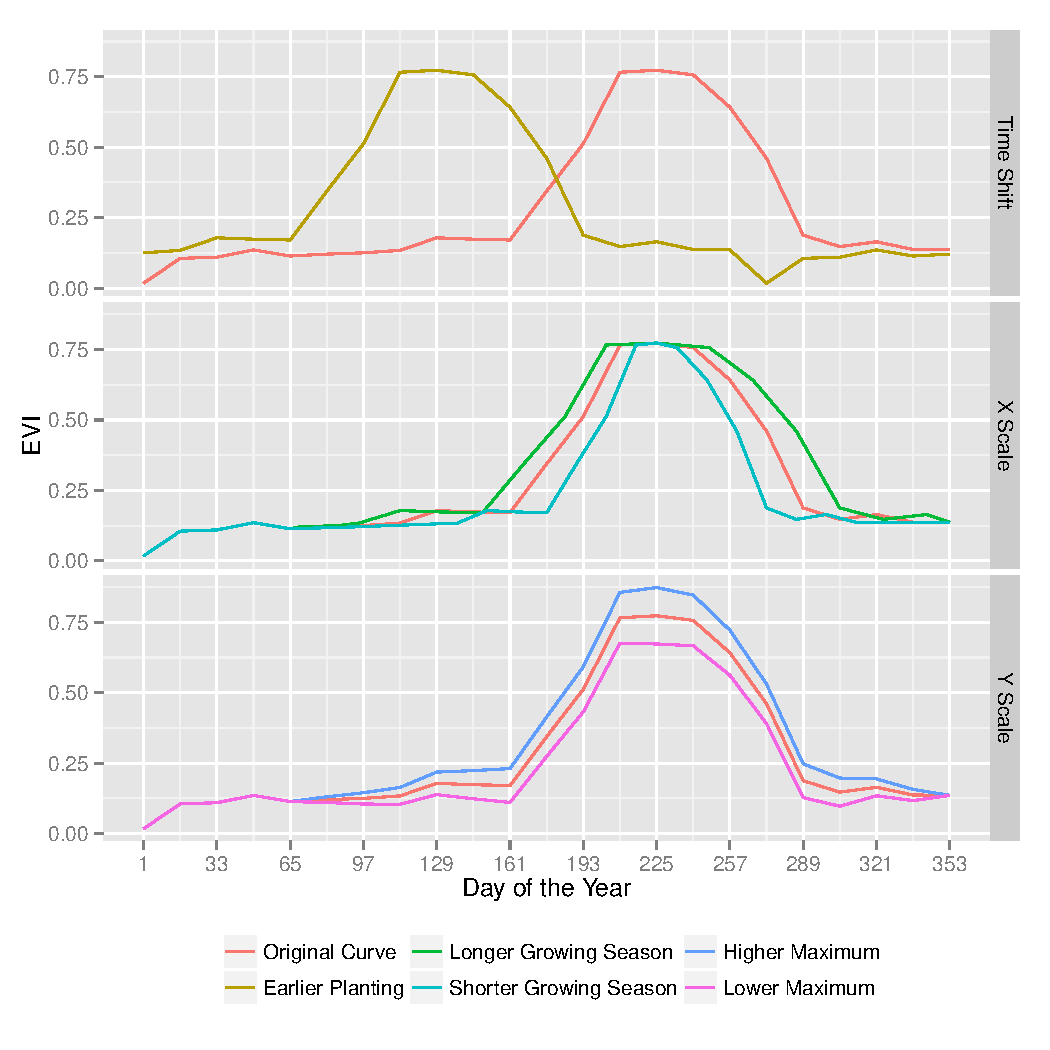
\includegraphics[width=\textwidth]{Graphics/transformations.pdf}
  \caption{Examples of transformations of a crop's VI curve due to interannual variations in growing conditions. The original curve was derived from soy in southwestern Kansas. The other curves were arbitrarily adjusted to illustrate each of the possible transformations.}
  \label{fig:transformations}
\end{figure}

Even without a mechanism to account for interannual differences, \textcite{brown2007multitemporal} used crop phenologies derived from multiple years of data to test four phenological classification methods. The authors fit the known phenologies to the unknown phenologies from other years by comparing the VI values throughout the growing season. The degree of likeness between a known VI curve and the unknown VI curve determined the classification. They showed that the best of the four classification methods was to find the sum of the square errors between the known and unknown curves (the SSE method, pg. 131).

The similarities between the methods presented in \citeauthor{brown2007multitemporal} and hyperspectral remote sensing techniques are striking. Hyperspectral techniques compare known spectral \textit{signatures} from a signature library to the unknown pixel signatures in an image. One method, spectral feature fitting, uses a least-squares comparison reminiscent of SSE from\citeauthor{brown2007multitemporal} \autocites{solutions2013selected}{clark2003imaging}. The key difference between the two, besides comparing reflectance across time versus reflectance across the electromagnetic spectrum, is that spectral feature fitting does not require any training data from the processed image. All of the spectral signatures used for identification are from standardized spectral libraries, containing many spectra of different materials.

Accordingly, one goal of this study is to realize a method of vegetation classification using multi- or hyper-temporal imagery that does not require training data to be extracted from the imagery itself, rather relying on standard libraries of \textit{temporal} signatures for different vegetation and non-vegetation land covers. A major challenge of this idea is that, unlike spectral signatures, temporal signatures are not necessarily consistent location to location, nor year to year as mentioned above. A viable classification method thusly must provide a way to transform the temporal signatures, within appropriate bounds, to match the horizontal scaling, vertical scaling, and time shifting of an unknown pixel before finding the degree of fit between the signature curve and the pixel curve.

\textcites{sakamoto2005a-crop}{sakamoto2010a-two-step} demonstrates a method using MODIS time-series data for use in finding key dates in a crop’s phenology, enabling better crop management strategies. Specifically, the authors’ two-step filter (TSF) method uses a wavelet transformation and a constrained minimization function to find a reference signature for a specific crop’s phenological development, and then fits that signature to known pixels of that crop type, finding the scaled dates of key transitions between developmental stages in the plants’ growth. This TSF method demonstrates that reference signatures can be fit to a pixel’s signature using a minimization function, accounting for the variations from the reference curve and the pixel curve.  This minimization method provides the means to account for the scaling and time shift differences, allowing previously-known temporal signatures (e.g. not from training sites) to be fit to pixel signatures in a VI TSI.

Specifically, from page 2151 of \textcite{sakamoto2010a-two-step}:
\begin{equation}
\label{eq:1}
  RMSE = \biggl[\frac{1}{365/s}\sum_{x=j(0), j(1)…}^{n}\bigl(f\left(x\right)-g\left(x\right)\bigr)^{2}\biggr]^{\frac{1}{2}}
\end{equation}
where $n$ is the number of dates in the TSI, $f(x)$ is the phenological curve for a given pixel in a dataset, and $x$ is the DOY, as defined by $j(y)$:
\begin{subequations}
\label{eq:DOYcalc}
  \begin{align}
    j\left(~y\right) &= k\bigl(~i\cdot~s\left(~y - 1\right)\bigr) \label{eq:jofy}\\
    \text{where\ \ \ \ } k\left(~z\right) &=
    \begin{cases}
      z, & \mbox{if } z \leq 0\\
      \left(z\bmod~365\right)\bmod~i-1, & \mbox{if } z > 0
    \end{cases} \label{eq:kofz}
  \end{align}
\end{subequations}
such that $s$ is the interval of the imagery and $d$ is the starting date of the imagery. $g(x)$ in Equation \ref{eq:1} is given by:
\begin{equation}
\label{eq:gofx}
  g(x) = yscale\times~h\left(xscale\times(x + tshift)\right)
\end{equation}

Here, $x$ again is the DOY, $yscale$ and  $xscale$ are coefficients controlling the vertical and horizontal scaling of a reference signature $h(x)$, and $tshift$ is a constant representing the horizontal shift, in days, of $h(x)$ (see Fig. \ref{fig:transformations}). Thus, if we minimize Equation \ref{eq:1} bounding $yscale$, $xscale$, and $tshift$  in $g(x)$ with reasonable values for each, we can calculate how well a given reference temporal signature $h(x)$ can be made to fit the pixel signature $f(x)$. Comparing a pixel's RMSE fit value from each of the reference signatures allows final classification; the signature with the lowest RMSE value has the best fit, and, of the tested signatures, provides the most probable identification.

\section{Field Methods and Data Collection in Pellegrini}

While ground truth data was easily available for the Kansas study site, getting a ground truth dataset for verification of the classification in Pellegrini was not so simple. Such a dataset did not exist, necessitating onsite data collection. I visited Argentina mid-March to early April 2014 to gather field observations of summer crop types and to talk to local farmers about typical agricultural practices, summer and winter crop varieties, and planting and harvesting dates.

To guide my ground truth collection, I generated 400 random points inside the Pellegrini shapefile boundary. Where a point fell within a mixel, I allowed it to be moved within a 3-by-3 pixel window centered on the point's original pixel, trying as much as possible to keep the point within a pixel belonging to the feature type on which it originally fell. In certain limited cases, if a point fell quite obviously within a field but the center pixel and eight surrounding pixels were mixels and/or were not within the field, I allowed the point to be moved to the closest full pixel of the same continuous field. Of the 400 points, I had move 106 within the 3-by-3 window, and ten to a non-neighboring pixel within the same field.

The primary means of gathering the crop identities to complete the ground truth was direct observation. However, this strategy proved to be difficult in many cases; often, fields were not accessible due to road conditions or locked gated. Data not from direct observations came from interviews with farmers and land owners. In such cases, the interviewees were asked to identify their fields on printed maps and describe their cultivars. The data from observations and interviews was recorded directly on the maps and later manually digitized.

Ancillary information about agricultural practices in the region was also collected whenever possible. It was a key goal to identify each crop's date range for planting and harvesting in order to allow the proper selection of MODIS imagery dates and setting of the $tshift$ bounds for Equation \ref{eq:gofx}.

\section{Data Processing}

\subsection{Resampling the CDL}

To use the CDL as a ground truth with the Kansas TSI, the 30-meter CDL pixels were resampled by majority to match the larger TSI pixels. This allowed a direct comparison between the crop values from the CDL and the pixel signatures in the TSI.

\subsection{Eliminating Mixels}

After building the TSIs, the next processing step was to eliminate mixels from the TSIs, to prevent errors caused by mixed temporal signatures (see Appendix \ref{appendix:testing:r2} for more information). Pure pixels, the non-mixels in the image, were isolated by intersecting the ground truth datasets with a vector grid of the TSI pixels. All pixels with an area greater than a certain area threshold were then selected as pure. I also manually selected two sorghum pixel features that were omitted due to intermixed soy pixels. I chose to add these pixels due to the low number of sorghum features retained, and that the intermixed soy appeared to be errors. Only these pure pixels were classified; the mixels in the images were ignored.

The original 30-meter CDL raster served as the reference for finding the pure pixels in the Kansas study site. The raster was converted to vector polygons and intersected with the TSI grid polygons. From the resulting geometry, all polygons greater than 53,000 square meters (or 98 percent of a full MODIS pixel) were selected as pure.

For the Argentina analysis, the digitized features of identified fields were combined with manually digitized features of all large forested areas, unknown fields, and ``other'' areas. Some places where the land cover was mixed and could not be visually differentiated were not digitized and were considered to be composed entirely of mixels. The complete dataset of land cover was then intersected with the Argentina TSI grid. Through trial and error, a minimum area of 50,000 square meters was used to select the pure pixels in the image.

\subsection{Extracting the Reference Temporal Signatures}

As a reference library of temporal signatures does not yet exist, I had to extract my own signatures from the Kansas TSI. To do so, the pure TSI pixels of each key summer crop---corn, soy, and sorghum---as specified in the resampled CDL were isolated in separate rasters. Each of separated rasters was clustered into three clusters using the ENVI \todo[inline]{Cite ENVI} k-means tool with a 1.0 percent change threshold over 100 maximum iterations. The TSI pixels in each cluster were then sampled and averaged to find the three primary signatures for each crop\footnote{Given the existing literature about phenological classification, I do not believe crops have multiple signatures. I believe every crop as a theoretical ideal signature, which can be made to fit any actual signature using the $xscale$, $yscale$, and $tshift$ transformations in Equation \ref{eq:gofx}, barring any unusual effects of weather or other forces impacting crop development (a mid-season drought, for example, may cause a crop signature with double peaks due to the partial dying off and regeneration of the plants). However, given my choice of the CDL as my source of ground truth, I have had to make the assumption that it is highly accurate, despite any evidence to the contrary (see my discussion of the CDL beginning in Appendix \ref{appendix:testing:r3}). Therefore, I use the clustering to derive the signatures that will create a classification most comparable to the CDL.} see Appendix \ref{appendix:tools:extract} for information about the Extract Signatures Tool).

\subsection{Fitting the Reference Signatures to the TSIs}

Equation \ref{eq:1} was implemented in Python with a command line interface to allow easy processing of the TSIs. Details of the tool can be found in Appendix \ref{appendix:tools:fit}. The tool iterates through every pixel in a TSI, comparing each reference signature with the pixel signature. An output raster is created for each signature to record the RMSE from every pixel comparison.

The reference signatures extracted from the Kansas TSI clusters were fit to the TSI to verify the classifier. Then, the same Kansas signatures were fit to the Pellegrini TSI. The fit rasters from each TSI were then classified. 

\subsection{Classifying the Fit Rasters}

The classification process is complex; Appendix \ref{appendix:tools:classify} contains a full discussion of the process, so I will refrain from a lengthy description here.

Classifying the fit rasters first requires thresholding the values in each raster, then finding the lowest value for each pixel. The signature with the lowest thresholded fit value has the best fit, and the pixel is classified as that crop. The thresholding prevents pixels with poor fit values from being classified as a crop. If a pixel has no remaining fit values after thresholding, it is classified as ``other.'' Currently, appropriate threshold values are not well understood, so to find the best classification, the classification tool must brute-force through many combinations of thresholds within a user-specified range, classifying the fit rasters, and calculating the accuracy of each threshold combination in comparison with the ground truth dataset. A raster of the classification with the best accuracy is retained.
























